\documentclass{beamer}

\usetheme{Madrid}
\setbeamertemplate{navigation symbols}{}

\usepackage{graphicx}
\DeclareGraphicsExtensions{.pdf,.png,.jpg}
\graphicspath{ {./img/} }

\usepackage{amsmath}
\usepackage{mathtools}

\title[Features]{Comparison of different Features Detectors and Descriptors in the Cut-Copy Forgery scenario}
\institute[CSI 445]{
    CSI 445 - Digital Image Forensics
}
\author[Seraphini,Teixeira]{Sibelius Seraphini, Larissa Teixeira}
\date{}

%\usetheme{Warsaw}

\begin{document}

    \frame{\titlepage}

    \begin{frame}
        \frametitle{Introduction}
        \begin{itemize}[<+->]
            \item Copy-move attacks
            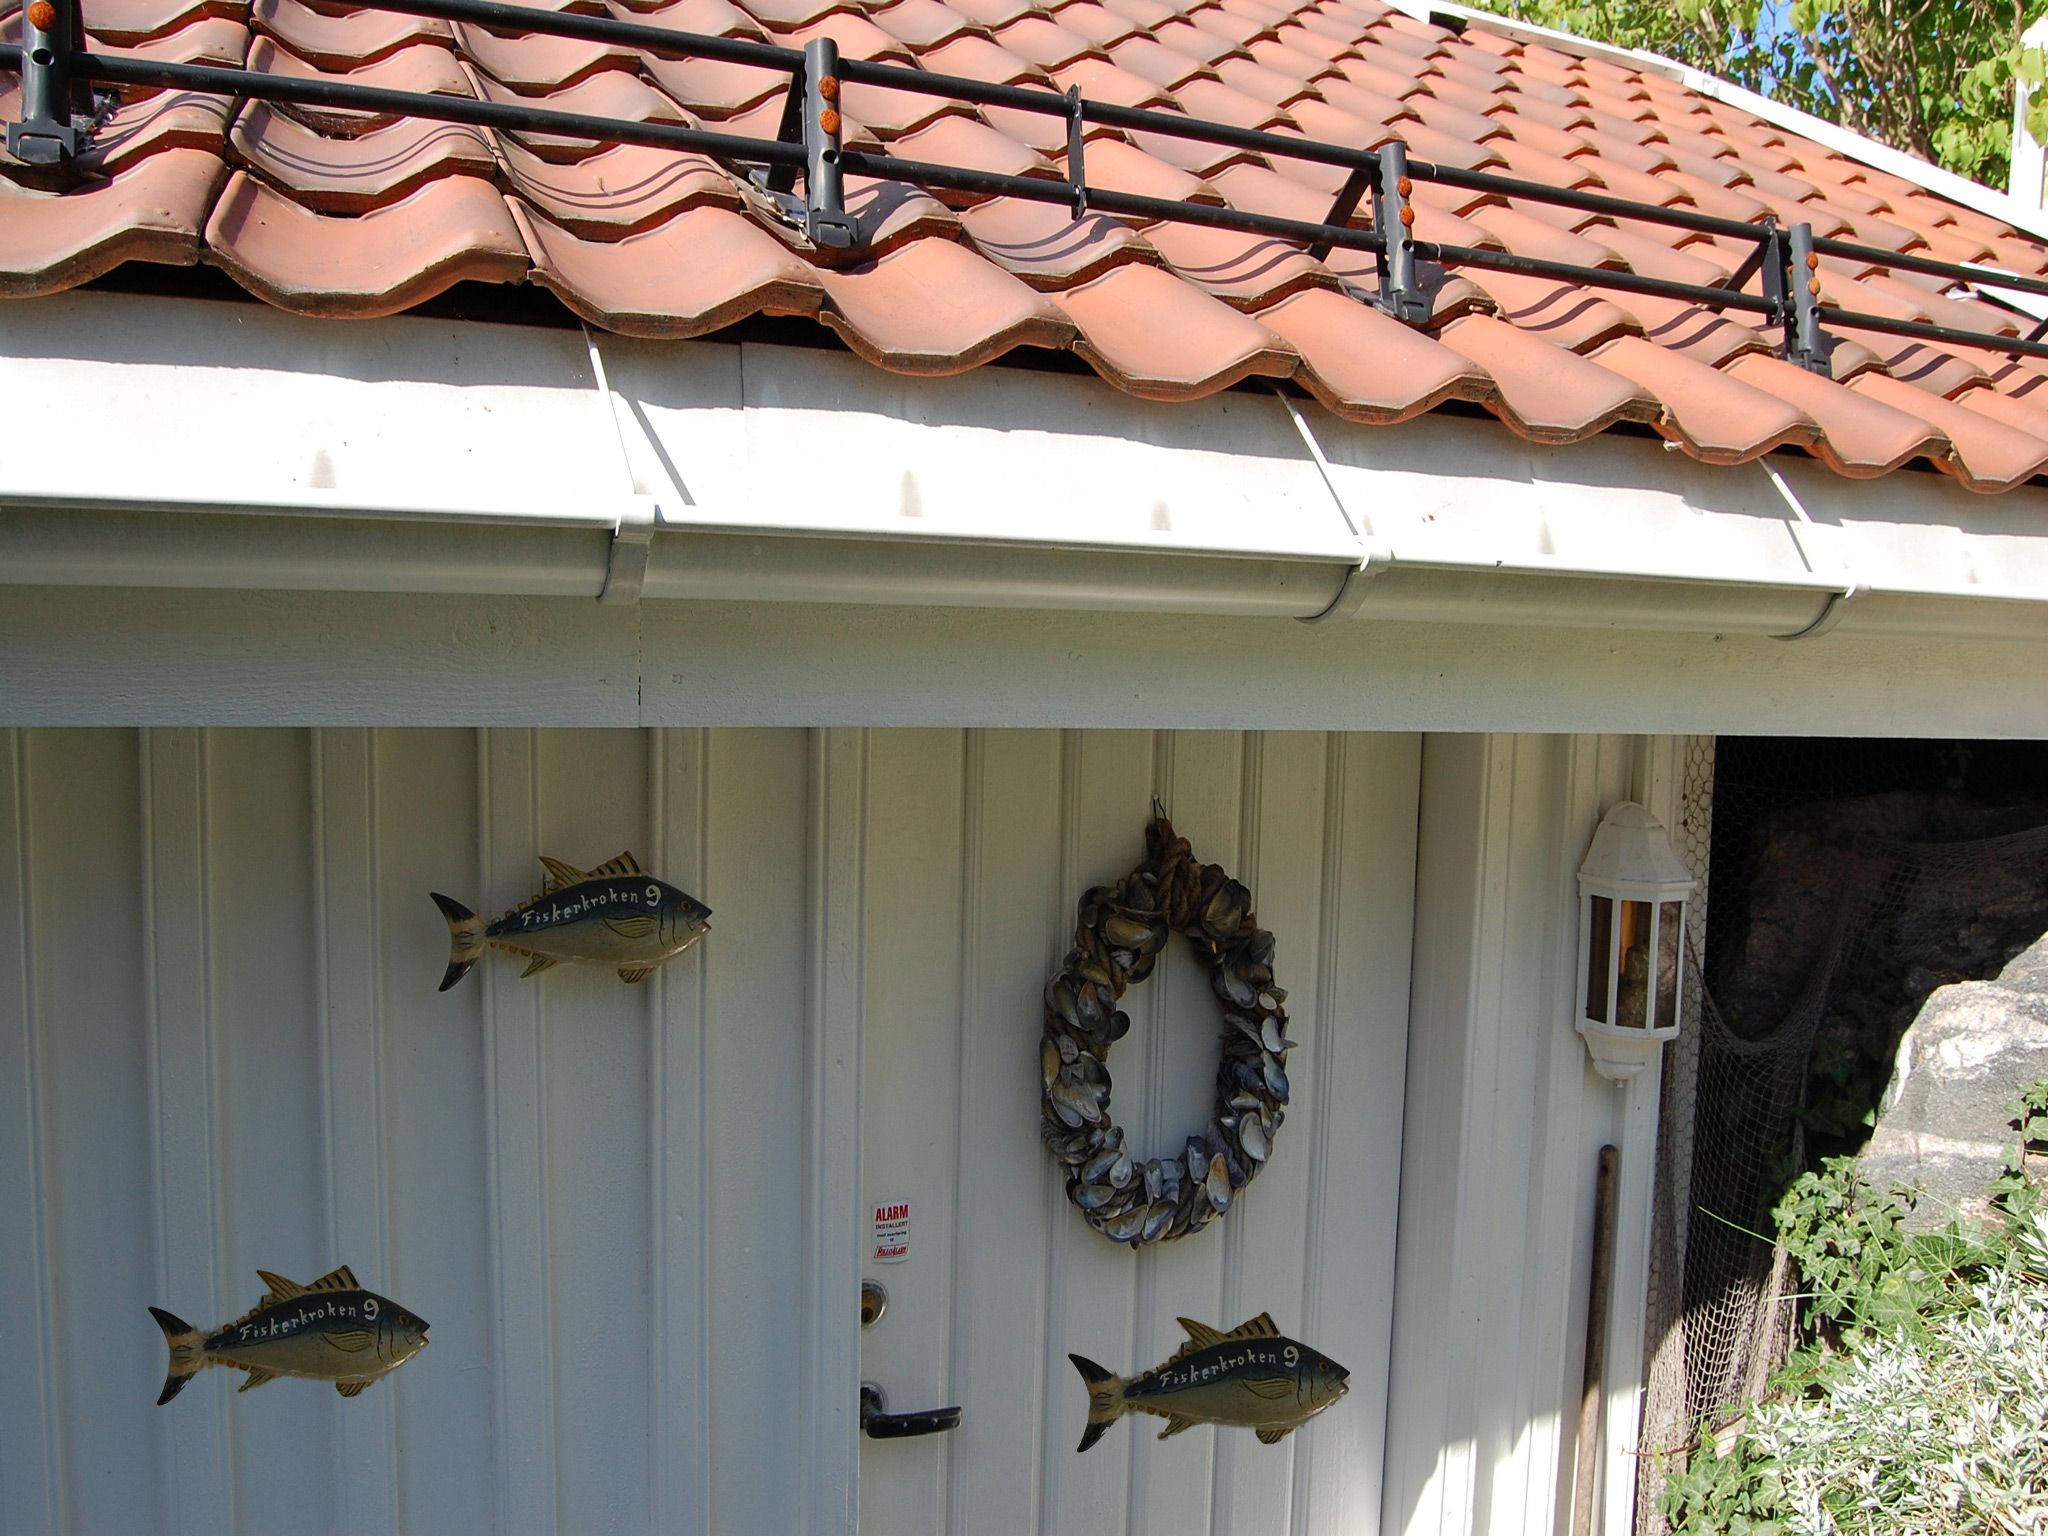
\includegraphics[width=10cm]{tamp}
        \end{itemize}
    \end{frame}

    \begin{frame}
        \frametitle{Motivation}
        \begin{itemize}
            \item What is the feature that better perform?
            	\begin{itemize}
                    \item What is the best KeyPoint detector?
                    \item What is the best KeyPoint descriptor?
                    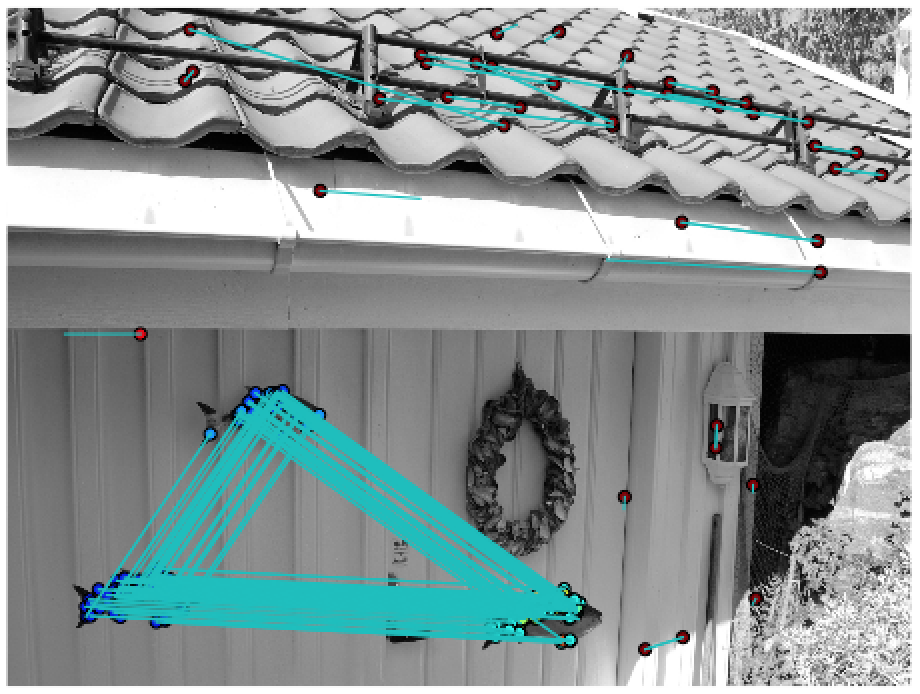
\includegraphics[width=8cm]{detected}
                \end{itemize}
        \end{itemize}
    \end{frame}

    \begin{frame}
        \frametitle{Methods}
        \begin{itemize} [<+->]
            \item Resource
                \begin{itemize}
                    \item Python
                    \item Numpy
                    \item Matlab
                    \item Opencv
                \end{itemize}
            \item Feature Detector
                \begin{itemize}
                    \item SIFT, SURF, STAR, ORB
                    \item BRIEF, BRISK, FREAK
                \end{itemize}
        \end{itemize}
    \end{frame}
    
    \begin{frame}
      \frametitle{Method}
      \begin{itemize}
            	\item Database - MICC-F220
        		\begin{itemize}
            		\item 220 images
			\item 82 tampered
			\item 83 original
        		\end{itemize}
	\end{itemize}
    \end{frame}

    
     \begin{frame}
      \frametitle{Related Work}
        \begin{itemize}
            	\item Features detection and matching
		\item Clustering and Forgery Detection
		\item Geometric Transformation Estimation
        \end{itemize}
    \end{frame}

    \begin{frame}
        \frametitle{Process}
        \begin{itemize}[<+->]
            \item Using a combination of each keypoint detector and descriptor
            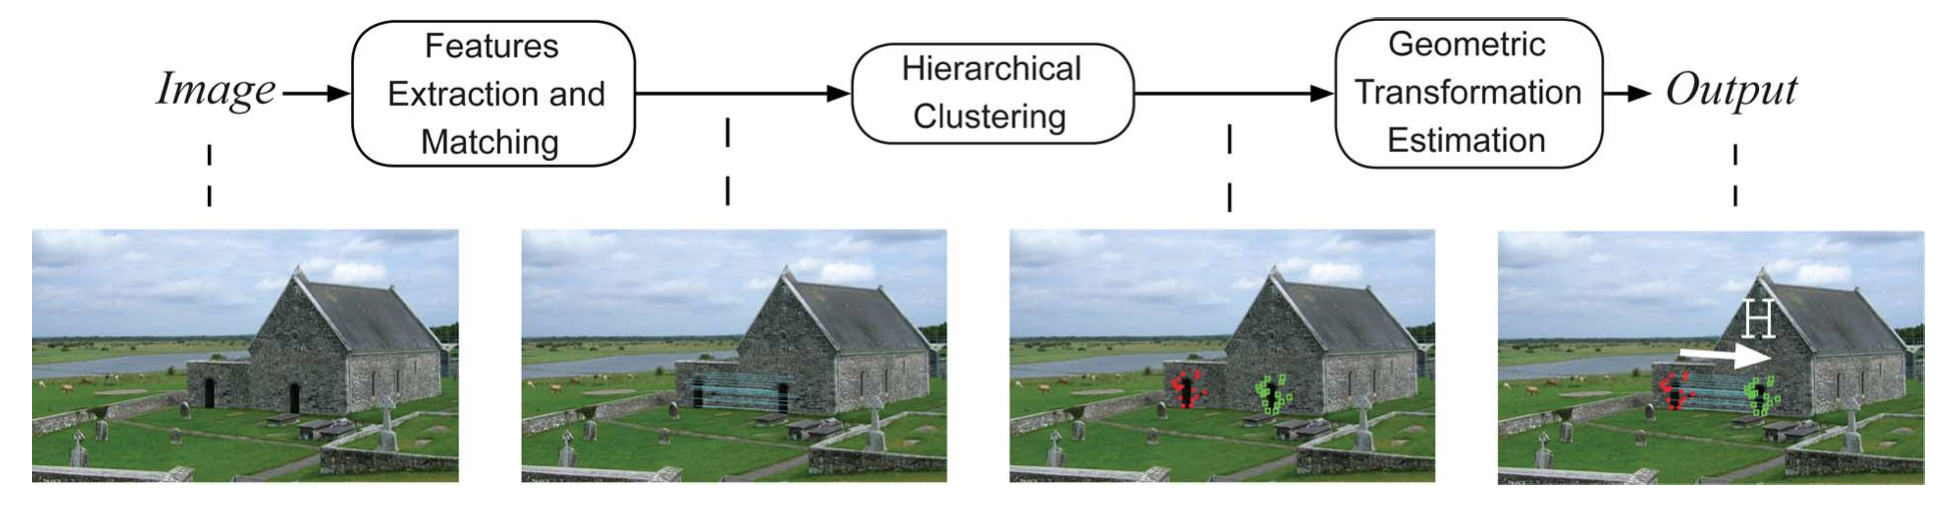
\includegraphics[width=10cm]{process}
        \end{itemize}
    \end{frame}

    \begin{frame}
        \frametitle{Results}
        \begin{itemize}[<+->]
            \item Table of Results
            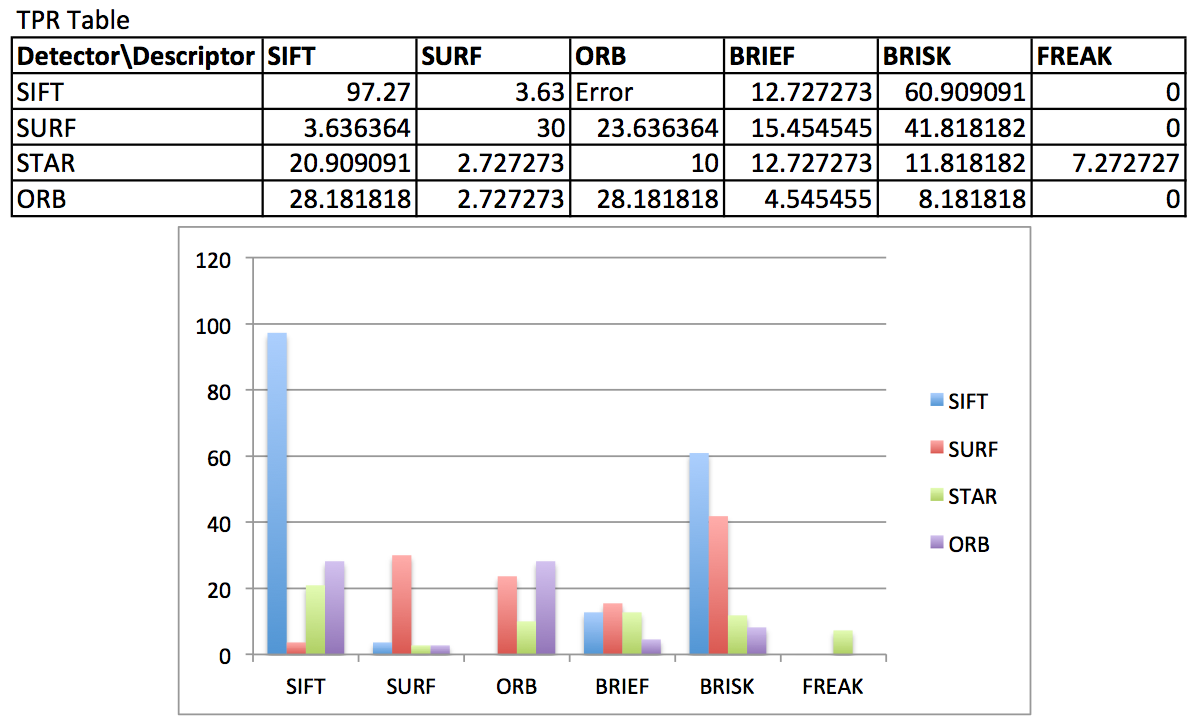
\includegraphics[width=10cm]{results_tpr}
        \end{itemize}
    \end{frame}
    
    \begin{frame}
        \frametitle{Results}
        \begin{itemize}[<+->]
            \item Table of Results
            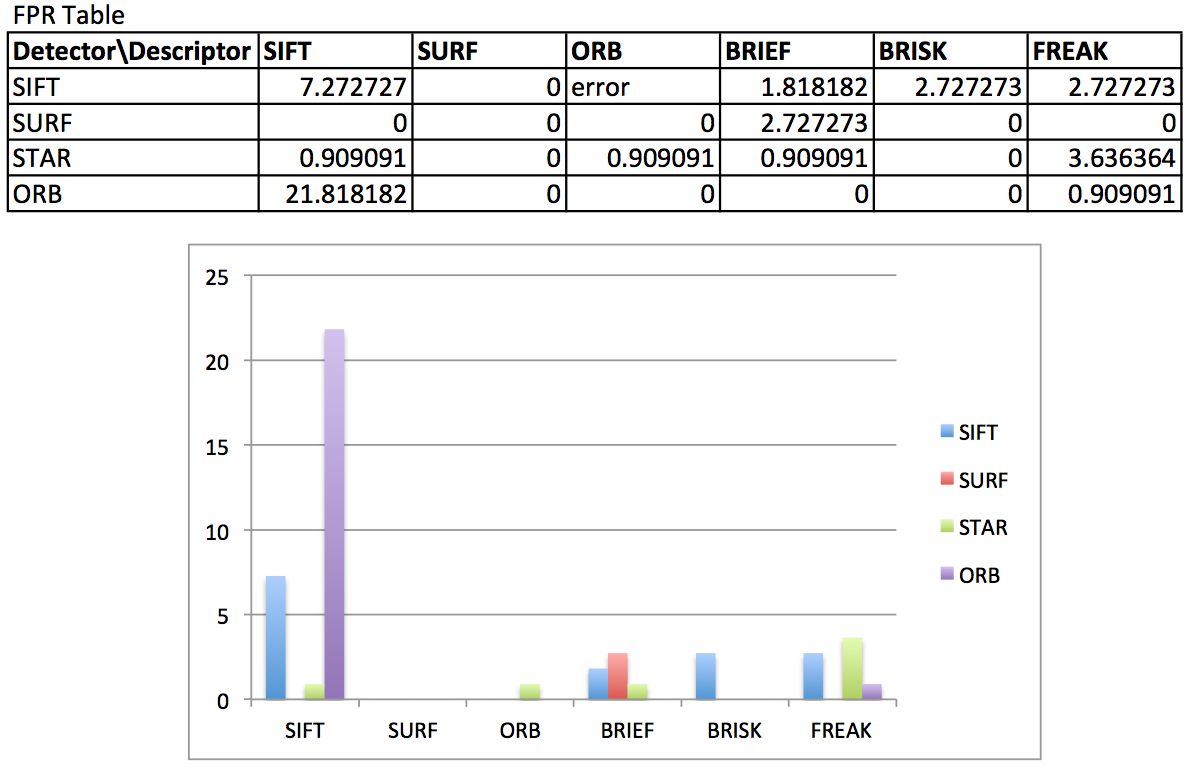
\includegraphics[width=10cm]{results_fpr}
        \end{itemize}
    \end{frame}
    
    \begin{frame}
        \frametitle{Results}
        \begin{itemize}[<+->]
            \item Table of Results
            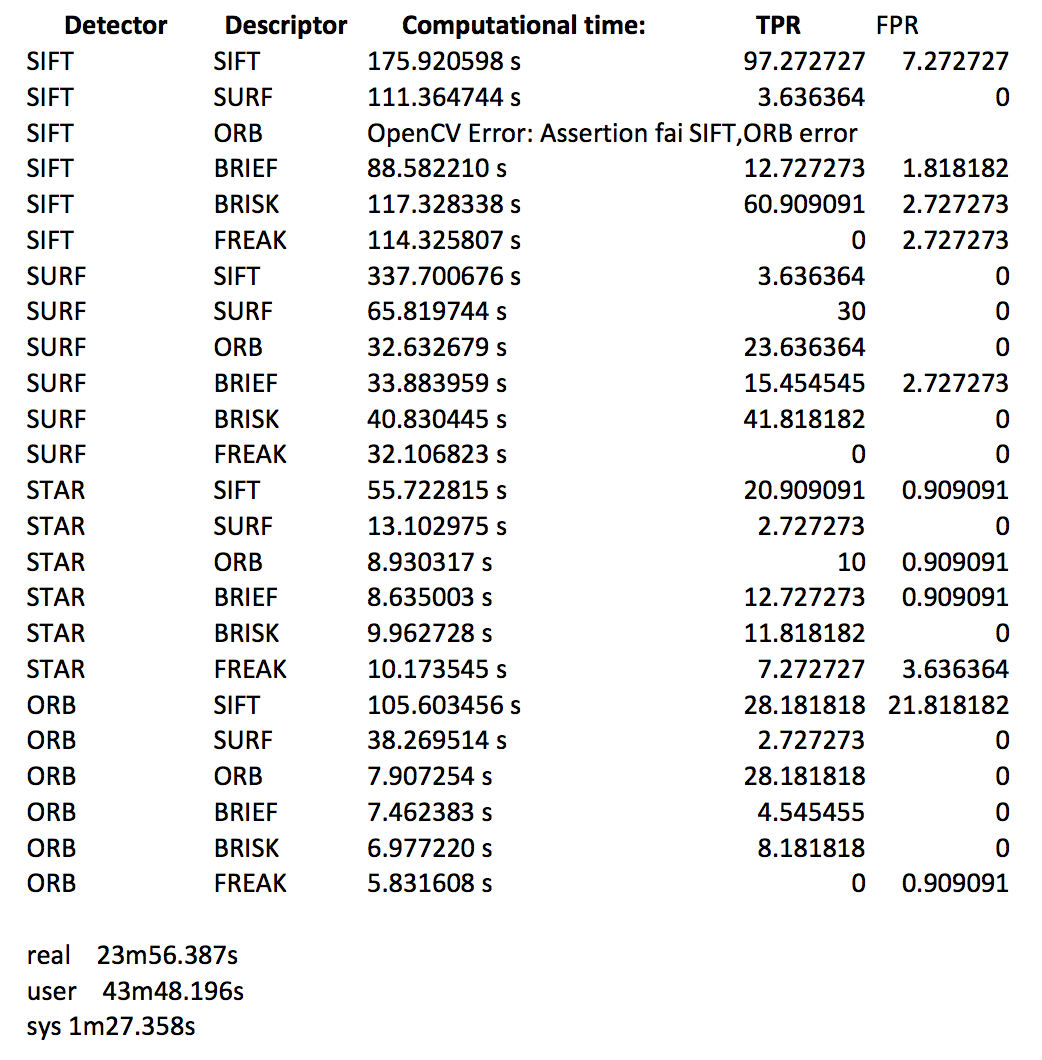
\includegraphics[width=10cm]{results_table}
        \end{itemize}
    \end{frame}
    
     \begin{frame}
        \frametitle{Rerefences}
        [1] Alahi, A., Ortiz, R., \& Vandergheynst, P. (2012, June). Freak: Fast retina keypoint. In Computer Vision and Pattern Recognition (CVPR), 2012 IEEE Conference on (pp. 510-517). IEEE.

[2] Amerini, I., Ballan, L., Caldelli, R., Del Bimbo, A., \& Serra, G. (2011). A SIFT-based forensic method for copy?move attack detection and transformation recovery. Information Forensics and Security, IEEE
Transactions on, 6(3), 1099-1110.

[3] Bay, H., Tuytelaars, T., \& Van Gool, L. (2006). Surf: Speeded up robust features. In Computer Vision?ECCV 2006 (pp. 404-417). Springer Berlin Heidelberg.

[4] Christlein, V., Riess, C., Jordan, J., \& Angelopoulou, E. (2012). An evaluation of popular copy-move forgery detection approaches. Information Forensics and Security, IEEE Transactions on, 7(6),
1841-1854.

[5] Lowe, D. G. (2004). Distinctive image features from scale-invariant keypoints.International journal of computer vision, 60(2), 91-110.

[6] Rublee, E., Rabaud, V., Konolige, K., \& Bradski, G. (2011, November). ORB: an efficient alternative to SIFT or SURF. In Computer Vision (ICCV), 2011 IEEE International Conference on (pp. 2564-2571).
IEEE.

    \end{frame}
  
    
    \begin{frame}
        \frametitle{Questions ?}
        \centering
        
\includegraphics[height=9cm]{questions}
    \end{frame}

\end{document}
